\phantomsection\label{doc:dee}

\section{Pulse calibration}
\label{sec:dee_pulse-calibration}
For an ideal resonant two-level drive, the target rotation is


\begin{equation}
    R_x(\theta)=\exp[-i\theta\sigma_x/2].
    \label{eq:dee_1}
\end{equation}


The rotation in \hyperref[eq:dee_1]{Eq.~(\ref*{eq:dee_1})} is the reference operation in this illustrative example \cite{nielsenQuantumComputationQuantum2010}.

As shown in \hyperref[fig:dee_1]{Fig.~\ref*{fig:dee_1}}, the Gaussian-shaped drive envelope is a schematic pulse, not experimental data.

\begin{figure}[H]
    \centering
    \ifdefined\mdToLatexCaptionBox\else\newsavebox{\mdToLatexCaptionBox}\fi
    \ifdefined\mdToLatexFigureHeight\else\newdimen\mdToLatexFigureHeight\fi
    \ifdefined\mdToLatexNaturalImageBox\else\newsavebox{\mdToLatexNaturalImageBox}\fi
    \setbox\mdToLatexCaptionBox=\vbox{
        \hsize=\linewidth
        \caption[Illustrative drive envelope]{\textbf{Illustrative drive envelope.} Normalized Gaussian-shaped pulse over a 20 ns window.}
        \label{fig:dee_1}
    }
    \sbox{\mdToLatexNaturalImageBox}{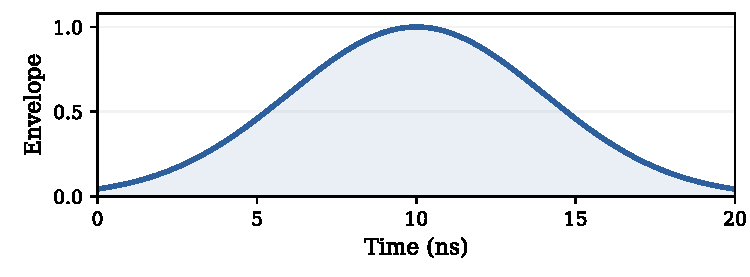
\includegraphics{Chapters/Figures/demo_pulse.pdf}}
    \mdToLatexFigureHeight=\dimexpr 0.96\textheight-\ht\mdToLatexCaptionBox-\dp\mdToLatexCaptionBox-\baselineskip\relax
    \ifdim\mdToLatexFigureHeight<1pt \mdToLatexFigureHeight=1pt\fi
    \ifdim\wd\mdToLatexNaturalImageBox>\linewidth
        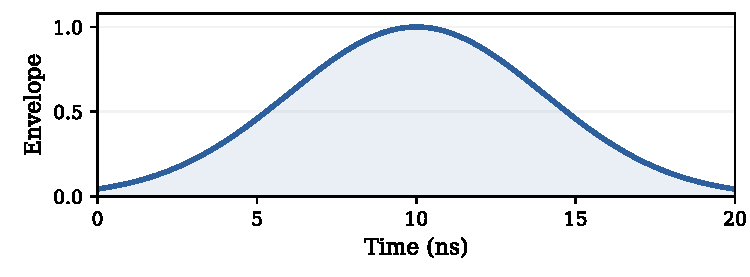
\includegraphics[width=\linewidth,height=\the\mdToLatexFigureHeight,keepaspectratio]{Chapters/Figures/demo_pulse.pdf}
    \else
        \ifdim\dimexpr\ht\mdToLatexNaturalImageBox+\dp\mdToLatexNaturalImageBox\relax>\mdToLatexFigureHeight
            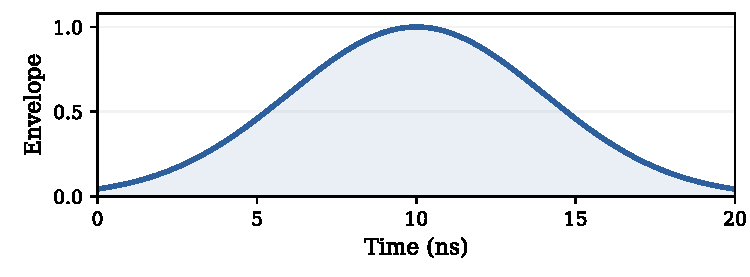
\includegraphics[width=\linewidth,height=\the\mdToLatexFigureHeight,keepaspectratio]{Chapters/Figures/demo_pulse.pdf}
        \else
            \usebox{\mdToLatexNaturalImageBox}
        \fi
    \fi
    \par\nobreak\noindent\usebox{\mdToLatexCaptionBox}
\end{figure}


The corresponding parameters are listed in \hyperref[tab:dee_1]{Table~\ref*{tab:dee_1}}.


\begin{table}[H]
    \centering
    \caption[Example pulse settings]{\textbf{Example pulse settings.} Illustrative values, not calibrated hardware parameters.}
    \label{tab:dee_1}
    \begin{tabular}{lr}
        \toprule
        \textbf{Parameter} & \textbf{Value} \\
        \midrule
        Pulse window & 20 ns \\
        Gaussian standard deviation & 4 ns \\
        \bottomrule
    \end{tabular}
\end{table}

